\chapter{Hello World}
\section{Providerwahl}
Wir haben uns für Swisscom als Provider entschieden, da es uns wichtig war, einen lokalen, heimischen Anbieter gezüglich Cloud Computing besser kennenzulernen. Swisscom ist in vielen Bereichen der IT und Telekommunikation schweizweit marktführend. 

In einem Gastvortrag an der HSR im Herbst 2016 ist ein Vertreter der Swisscom erschienen und hat von der Vorzügen und der gelebten Swissness erzählt. Da wir noch nie mit PaaS Produkten im Allgemeinen gearbeitet haben war dies die perfekte Möglichkeit um in die Thematik reinzufinden. 
\section{Anleitung}
Der Einstieg fiel allgemein gesehen leicht. Swisscom verwendet \glqq Cloud Foundry\grqq für ihre Application Cloud. Mittels Tutorials auf der Webseite wird man für den Einstieg gut \glqq an der Hand genommen\grqq .

\begin{longtable}{| p{5cm} | p{11cm} |}
\hline
Unter https://docs.developer.swisscom.com/getting-started/ 
findet man Tutorials für die verschiedenen PaaS Produkte wie z.B. Python, Java, Node.js
&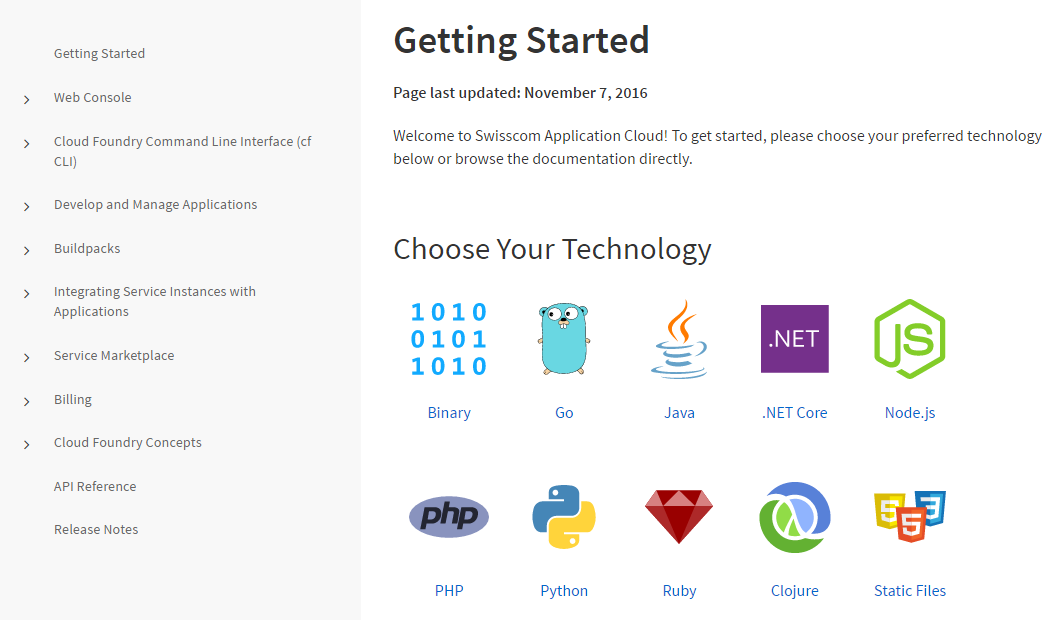
\includegraphics[width=0.65\columnwidth, valign=T]{images/image1.png}\\ \hline
Als allererstes benötigt man das Cloud Foundry Command Line Interface. Auf der Webseite sind Beschreibungen für die Installation unter Linux/Macintosh/Windows zu finden. (Windows in dieser Anleitung) 
&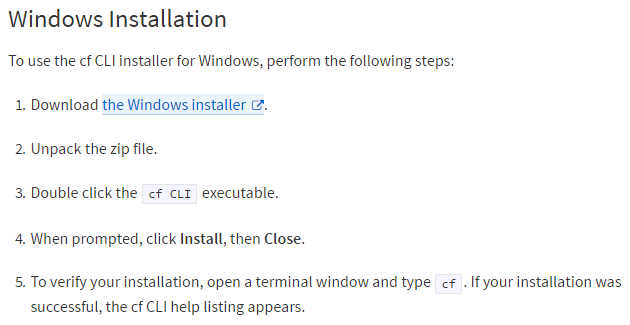
\includegraphics[width=0.65\columnwidth, valign=T]{images/image2.png} \\ \hline
Nach erfolgreicher Installation ist das „cf“-Tool per Windows Commandline (cmd) benutzbar&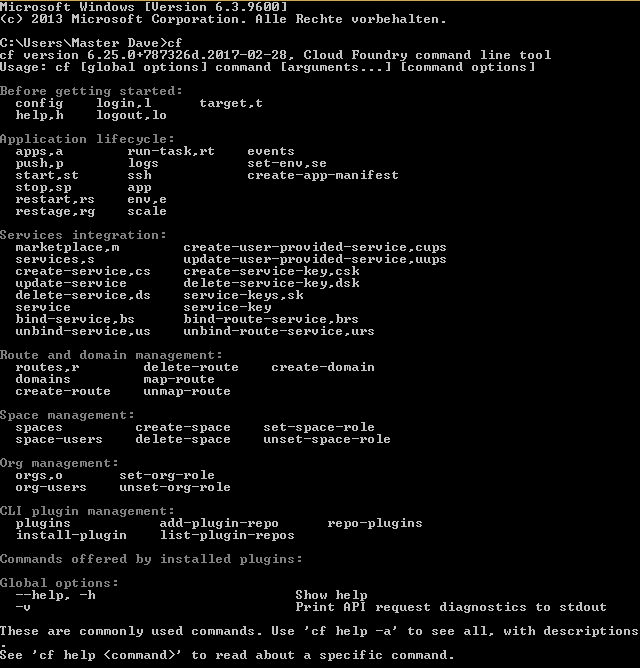
\includegraphics[width=0.65\columnwidth, valign=T]{images/image3.png} \\ \hline
Nun können wir uns mit der Web Console von der Swisscom App Cloud vertraut machen. Auch hier gibt es ein Tutorial 
&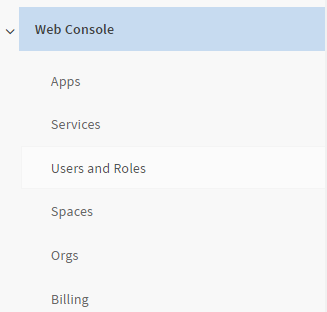
\includegraphics[width=0.65\columnwidth, valign=T]{images/image4.png} \\ \hline
Jetzt können wir das Tutorial für eine Java App durcharbeiten &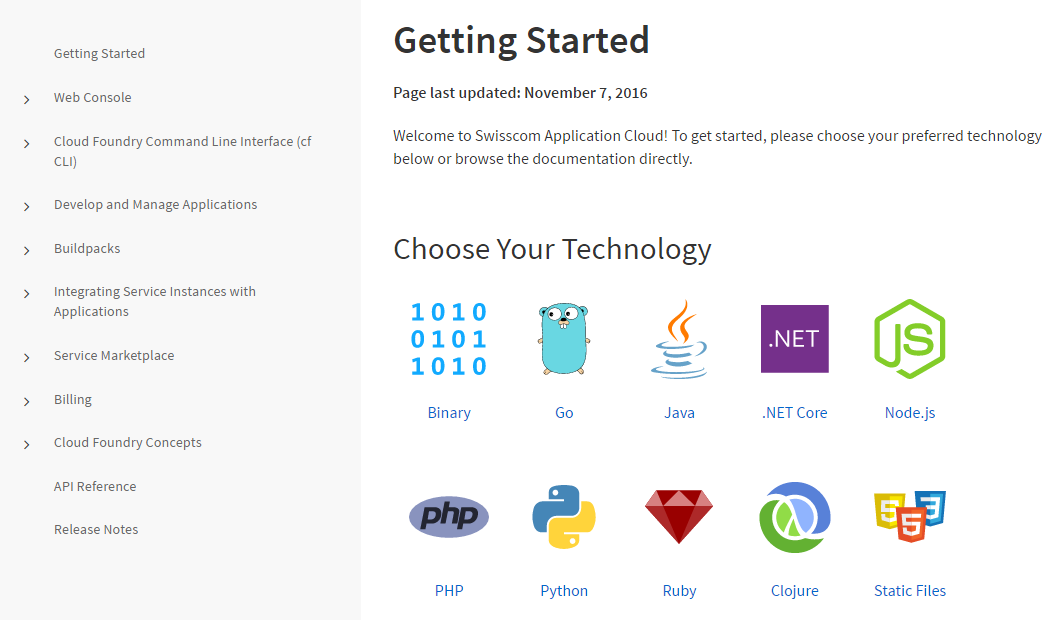
\includegraphics[width=0.65\columnwidth, valign=T]{images/image1.png} \\ \hline
Als Erstes sollte man die Prereqs überprüfen 
&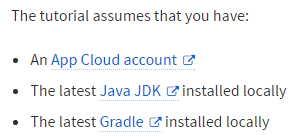
\includegraphics[width=0.65\columnwidth, valign=T]{images/image5.png} \\ \hline
Nun muss man sich über die cf Console an der Swisscom App Cloud anmelden. Wir skippen die Zuweisung an eine Org. 
&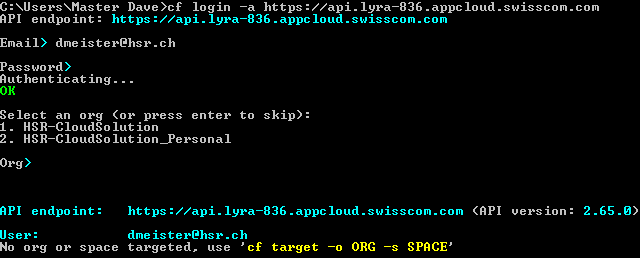
\includegraphics[width=0.65\columnwidth, valign=T]{images/image6.png} \\ \hline
Unter https://console.developer.swisscom.com erstellen wir eine neue Org Namens „HelloWorld“. &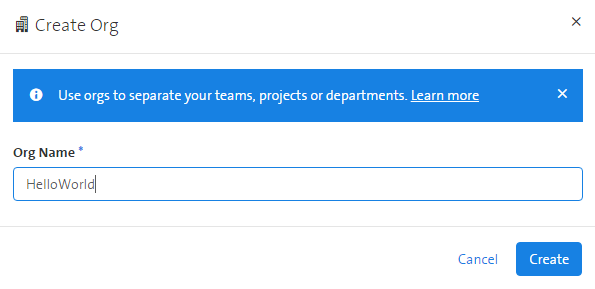
\includegraphics[width=0.65\columnwidth, valign=T]{images/image7.png} \\ \hline
In dieser Org müssen wir einen Space erstellen. 
&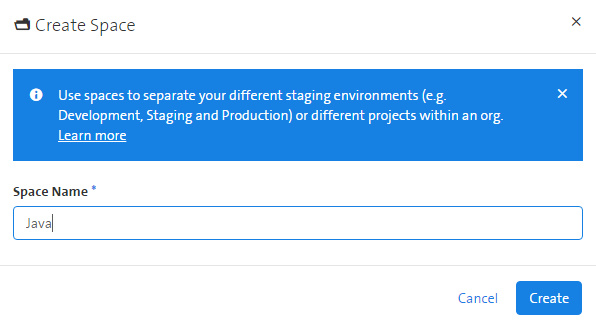
\includegraphics[width=0.65\columnwidth, valign=T]{images/image8.png} \\ \hline
Wir weisen nun Org und Space mittels „cf target –o HelloWorld –s Java“ zu &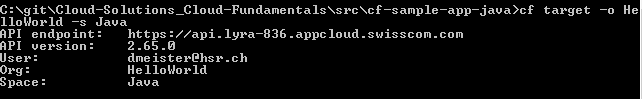
\includegraphics[width=0.65\columnwidth, valign=T]{images/image9.png} \\ \hline
Wir kopieren nun die Java Beispielapp von Swisscom 
&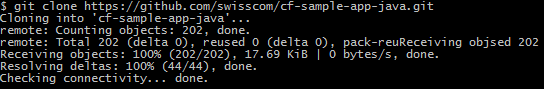
\includegraphics[width=0.65\columnwidth, valign=T]{images/image10.png} \\ \hline
Nun können wir mit Gradle die App builden. Es wurde ein jar generiert. &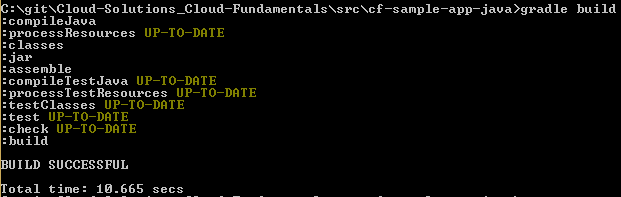
\includegraphics[width=0.65\columnwidth, valign=T]{images/image11.png} \\ \hline
Diese .jar File können wir nun mittels „cf push my-java-app“ –p <path to jar>„ –n „ pushen &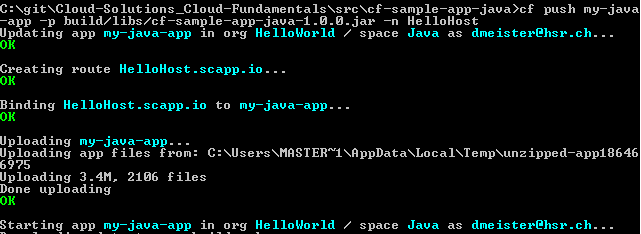
\includegraphics[width=0.65\columnwidth, valign=T]{images/image12.png} \\ \hline
Sobald die App erfolgreich gestartet wurde erscheinen folgende Meldungen &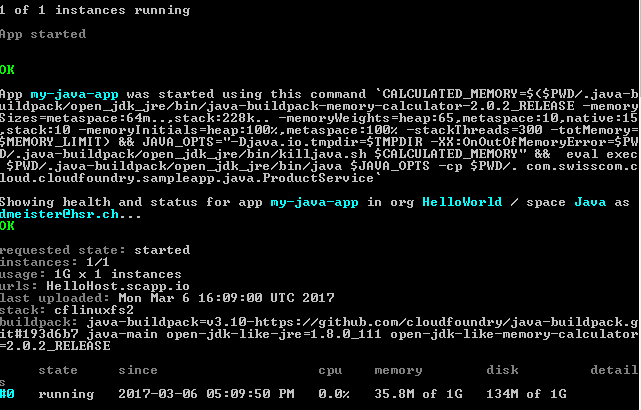
\includegraphics[width=0.65\columnwidth, valign=T]{images/image13.png} \\ \hline 
Mittels „cf app my-java-app“ kann man den Status der Java App abrufen &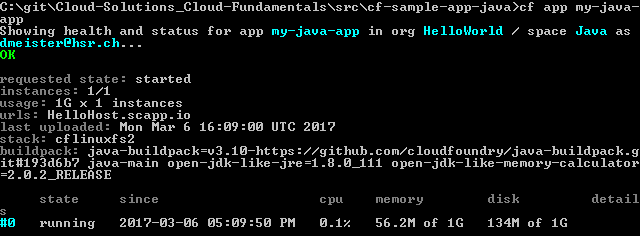
\includegraphics[width=0.65\columnwidth, valign=T]{images/image14.png} \\ \hline
Mittels „cf scale my-java-app“ erhält man eine Übersicht über die verwendeten Ressourcen Memory, Disk, Instances 
&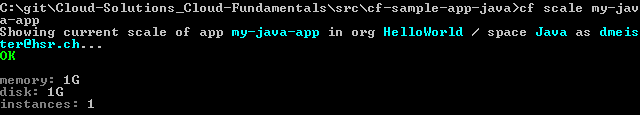
\includegraphics[width=0.65\columnwidth, valign=T]{images/image15.png} \\ \hline
Horizontales Scaling geschieht mittels „cf scale my-java-app –i 3“. So werden nun 3 Instanzen verwendet 
&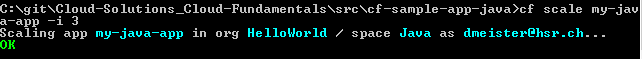
\includegraphics[width=0.65\columnwidth, valign=T]{images/image16.png} \\ \hline
Vertikales Scaling geschieht mittels „cf scale my-java-app –m 2G“. So werden 2 GB RAM verwendet &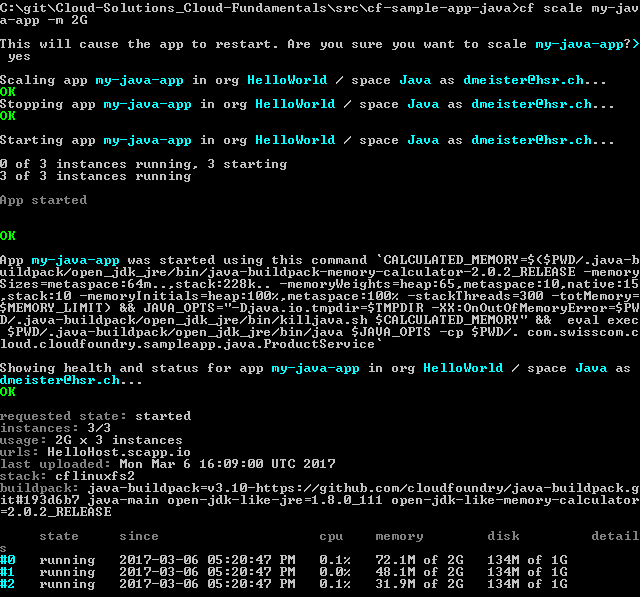
\includegraphics[width=0.65\columnwidth, valign=T]{images/image17.png} \\ \hline
Es gilt nun zu beachten, dass nach dem Scaling die Betriebskosten gestiegen sind. &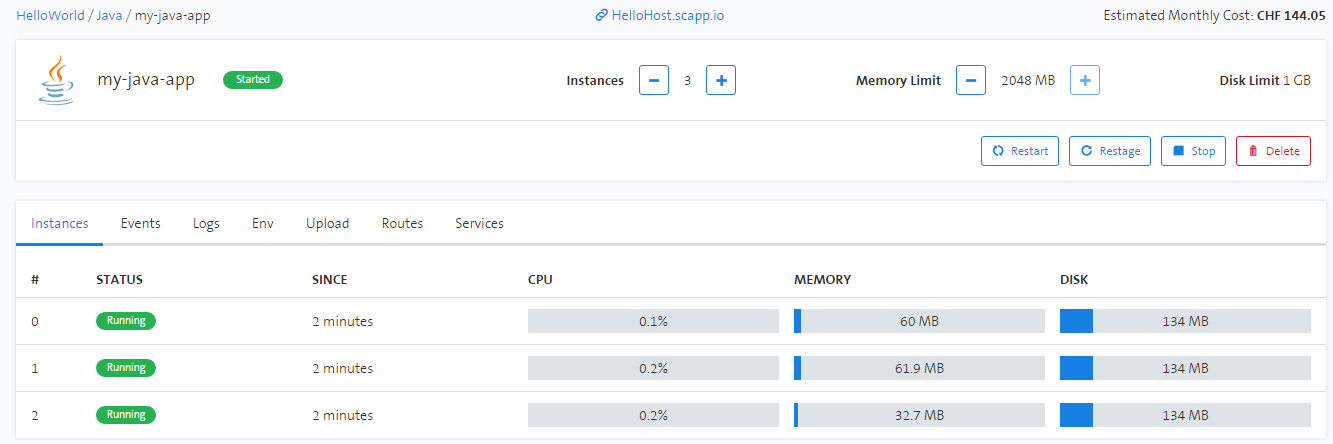
\includegraphics[width=0.65\columnwidth, valign=T]{images/image18.png} \\ \hline
Die Logfiles können einfach mittels „cf logs my-java-app --recent“ abgerufen werden &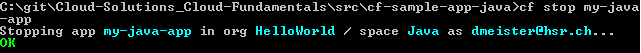
\includegraphics[width=0.65\columnwidth, valign=T]{images/image19.png} \\ \hline
Mittels „cf stop my-java-app“ kann die App gestoppt werden. Falls sie wieder benötigt wird kann sie mittels „cf start my-java-app“ wieder hochgefahren werden. 
&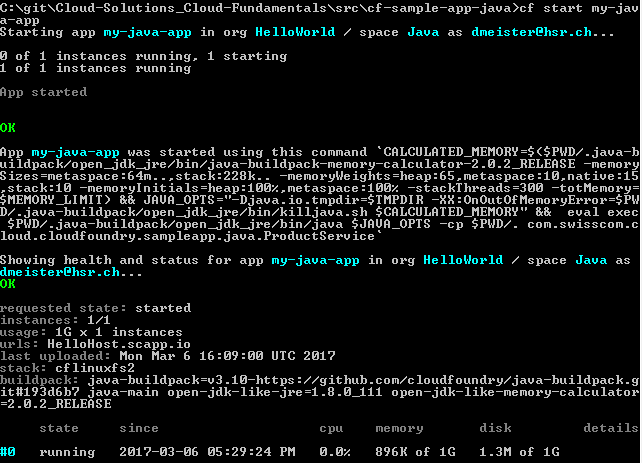
\includegraphics[width=0.65\columnwidth, valign=T]{images/image20.png} \\ \hline
\end{longtable}

\chapter{OSSM-Definition}
\section{On-Demand}
Es gibt mehere unterstütze Services und Programmiersprachen, die bereits Verfügbar sind. Nach der Anmeldung und der Angabe der Kreditkarte können solche Instanzen erstellt werden und sind ohne Wartezeiten einsatzbereit. Dies merkt der User durch die vorbereiteten Templates, welche er schnell erstellen und starten kann.
\section{Self-Service}
Es gibt viele verschiedene Templates, welche bereits Verfügbar sind. Diese können leicht mit der Weboberfläche erstellt werden. Der Entwickler pushed danach seine lokale Applikation via CLI auf diesen Webspace und die Applikation ist einsatzbereit.
\begin{figure}[H]
\centering
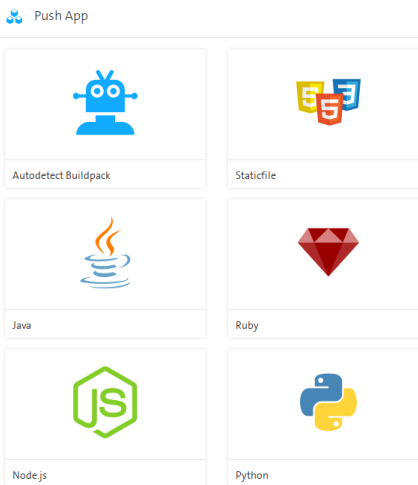
\includegraphics[scale=0.65]{images/image01.png} 
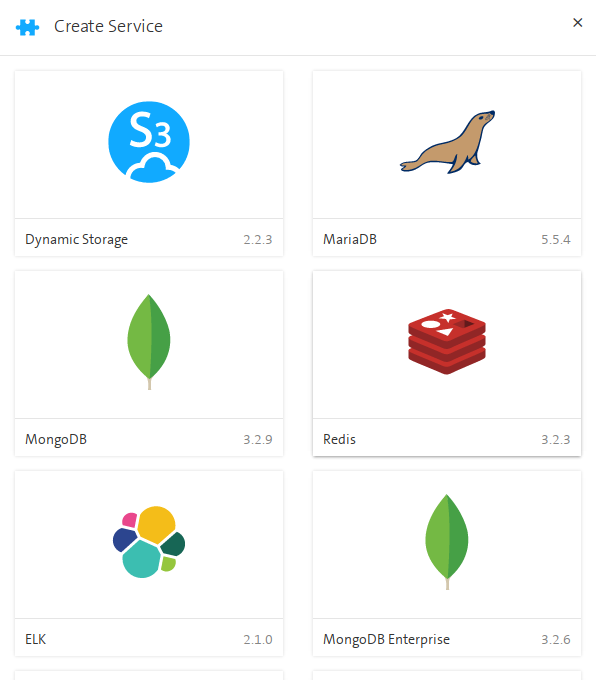
\includegraphics[scale=0.3]{images/image08.png} 
\end{figure}

\section{Scalable}
Jede Applikation kann man weitere Instanzen hinzufügen. Auch der maximale Arbeitsspeicher und der Festplattenspeicher kann eingestellt werden, doch es werden nur 2 GB Arbeitsspeicher unterstüzt. Der Festplattenspeicher aber nur über das CLI. Die Skalierung muss von Hand erledigt werden, da es keine Möglichkeit zur automatischen Skalierung gibt.
\begin{figure}[H]
\centering
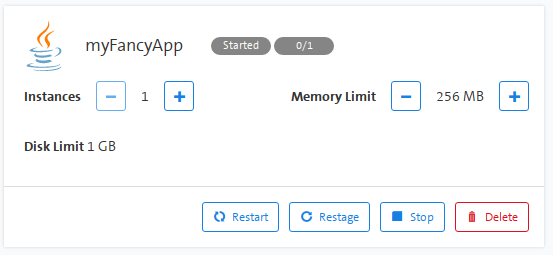
\includegraphics[scale=0.5]{images/image09.png} 
\end{figure}

\section{Measureable}
Bei der Cloudlösung der Swisscom sieht man die Kosten bereits beim Erstellen des Services. Dabei werden die Kosten aus der Anzahl Instanzen und der Arbeitsspeicherlimite berechnet. Gezahlt wird die monatliche Rechnung per Kreditkarte.
\begin{figure}[H]
\centering
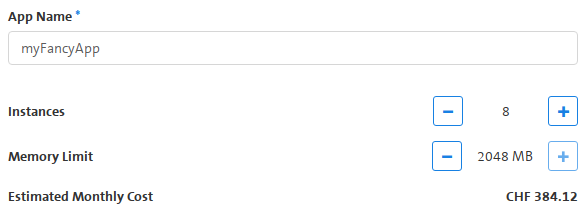
\includegraphics[scale=0.5]{images/image07.png} 
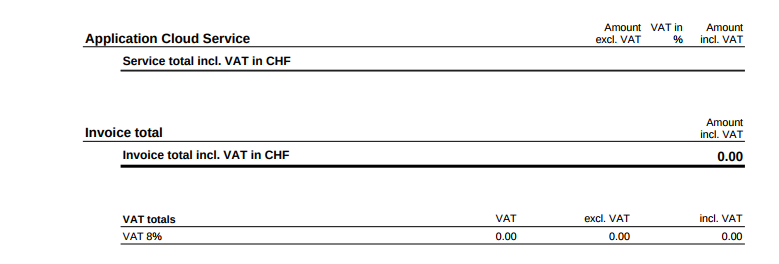
\includegraphics[scale=0.5]{images/image05.png} 
\end{figure}
\chapter{Cloud Computing Patterns}
Die Swisscom Application Cloud setzt das Service-Modell \glqq Platform as a Service\grqq (PaaS) um. Im Bild sind die drei vorgängigen Servicemodelle im Vergleich mit PaaS ersichtlich.
 
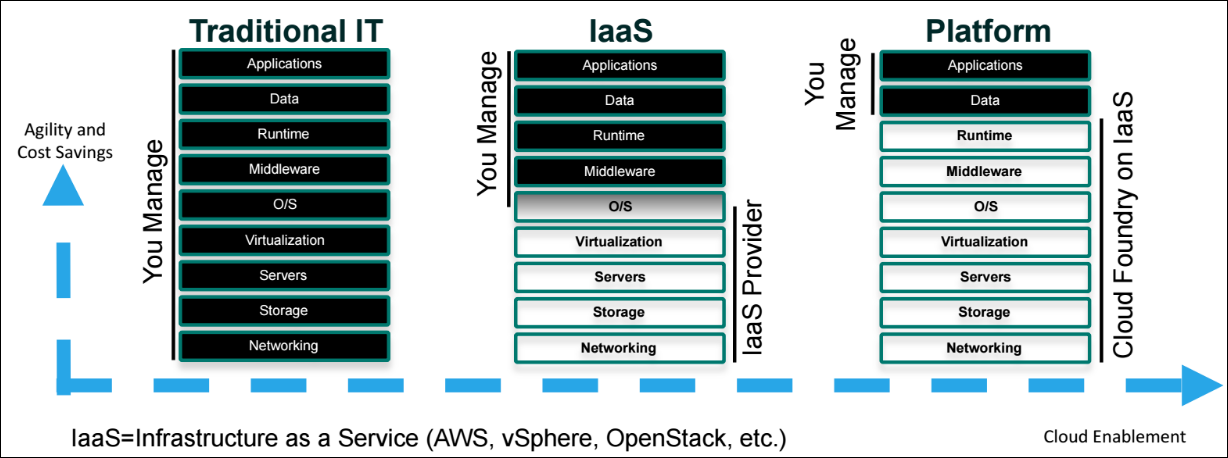
\includegraphics[scale=0.25]{images/power-of-platform.png}

Swisscom verwendet Cloud Foundry für ihre Application Cloud Plattform. Cloud Foundry wird ebenfalls von vielen anderen Providern und Firmen (z.B. IBM, Pivotal, SAP, usw.) verwendet sowie weiterentwickelt. Somit ist Cloud Foundry ein Open Source Projekt. Diese Konstellation verhindert Vendor-lock-ins, d.b. es sollte sehr einfach sein die Provider für die eigenen Enterprise Applikationen auszutauschen. Dies generiert für die Kunden einen echten Mehrwert.
 
\section{Process Offering}
Als Entwickler möchte man eine fix-fertige Umgebung aus einem Guss. Die Swisscom Application Cloud bietet deshalb fertige Umgebungen für Programmierer. 

Diese Anforderungen können mit dem Pattern \glqq Execution Environment\grqq umgesetzt werden.

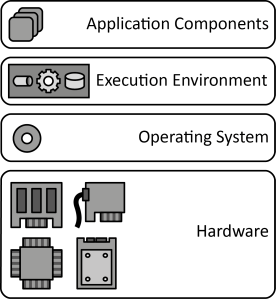
\includegraphics[scale=3]{images/execution-environment.png}

Für den Kunden ist vordergründig nicht viel sichtbar. Er kann seine Sources in die Cloud laden und von der Execution Environment ausführen lassen. Die App wird dann in einem Container ausgeführt und die darunterliegende Infrastruktur ist für den Kunden unbekannt. 

\section{Workload}
Bei der Swisscom Application Cloud wird kein Auto-Scaling unterstützt. Dies verhindert den Einsatz bei gewissen Workload Patterns. Man kann problemlos die Applikation skalieren, jedoch muss dies manuell geschehen. Eine häufige Änderung des Workloads ist daher ungeeignet. Deshalb fallen folgende Workload Patterns wohl nicht in das Aufgabengebiet der Swisscom Application Cloud:
\begin{itemize}
\item Periodic Workload
\item Unpredictable Workload
\item Continuously Changing Workload
\end{itemize}

Hingegen sind die Workload Patterns \glqq Static Workload\grqq und \glqq Once-in-a-Lifetime\grqq Workload gut geeignet.


\includegraphics[scale=0.6]{images/static-workload.png}

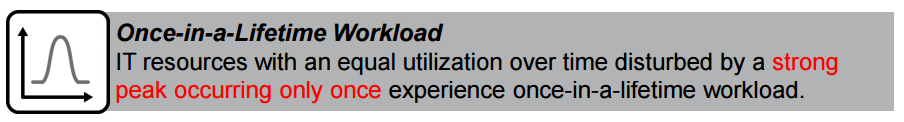
\includegraphics[scale=0.6]{images/once-lifetime.png}

Bei einer statischen Workload muss offensichtlich nicht skaliert werden. Bei Events, welche einmalig auftreten ist es ebenfalls kein Problem, dies manuell zu skalieren.

\section{Komponenten}
Das Angebot in der Swisscom Application Cloud kann in zwei Gruppen unterteilt werden:
\begin{itemize}
\item Applications
\item Services
\end{itemize}

Bei den Applications kann man als User seine Applikationen bereitstellen. Folgende Technologien stehen zur Verfügung:

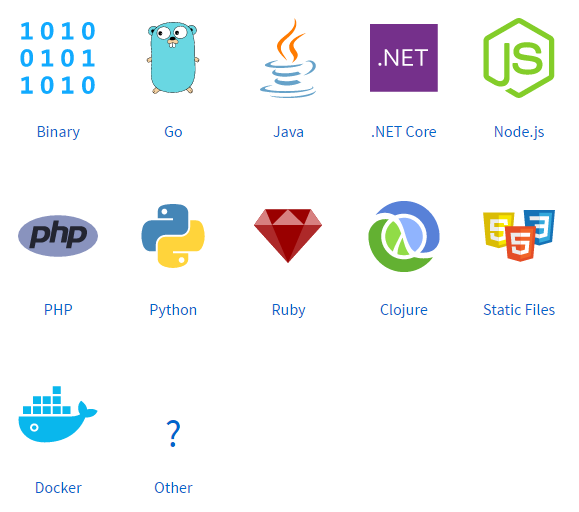
\includegraphics[scale=0.7]{images/applications.png}

Als Services stehen bekannte Produkte unterschiedlicher Hersteller bereit. Diese wären beispielsweise MongoDB als Vertreter der NoSQL Familie. MariaDB fungiert als SQL Datenbank und Redis als Key-Value Store. Für Queueing und Messaging steht RabbitMQ zur Verfügung. 

Swisscom Application Cloud stellt das CCP \glqq Execution Environment\grqq dem Kunden zur Verfügung. Hypervisor als Process Offering ist an dieser Stelle fehl am Platz da man auf einer höheren Abstraktionsstufe arbeitet. Die Hardware resp. Virtualisierungsplattform ist hier nicht ersichtlich, resp. Black-Box. 

Möchte man Map-Reduce Computing, so muss man sich selber darum kümmern, resp. es wird von Swisscom nichts out-of-the-box angeboten.

\section{Übersichtsgrafik}
Die Hello World Java App kann gemäss dem Pattern \glqq Elastic Platform\grqq platziert werden.

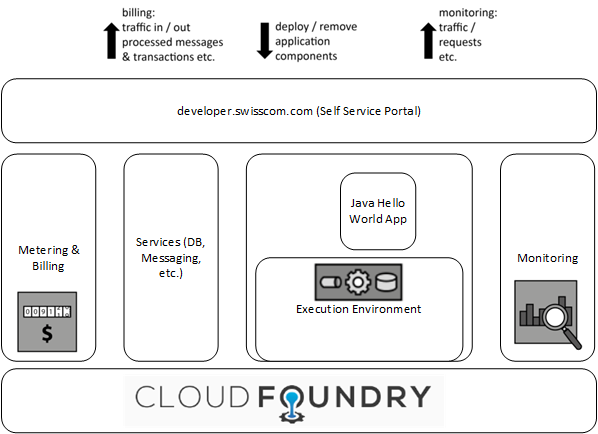
\includegraphics[scale=0.7]{images/visualisierung}



\chapter{Self-Information}
Bei der Installation gab es wenige Probleme. Hier sind die wichtigsten Schritte kurz aufgezeigt.
\begin{longtable}{| p{5cm} | p{11cm} |}
\hline
In IntelliJ importiert man sich das Projekt und lädt das Cloud Foundry Plugin herunter. Nun loggt man sich ein und erstellt eine Verbindung zu seiner Swisscom-Cloud. Die Organization und der Space werden nach dem Login sofort gefunden.
&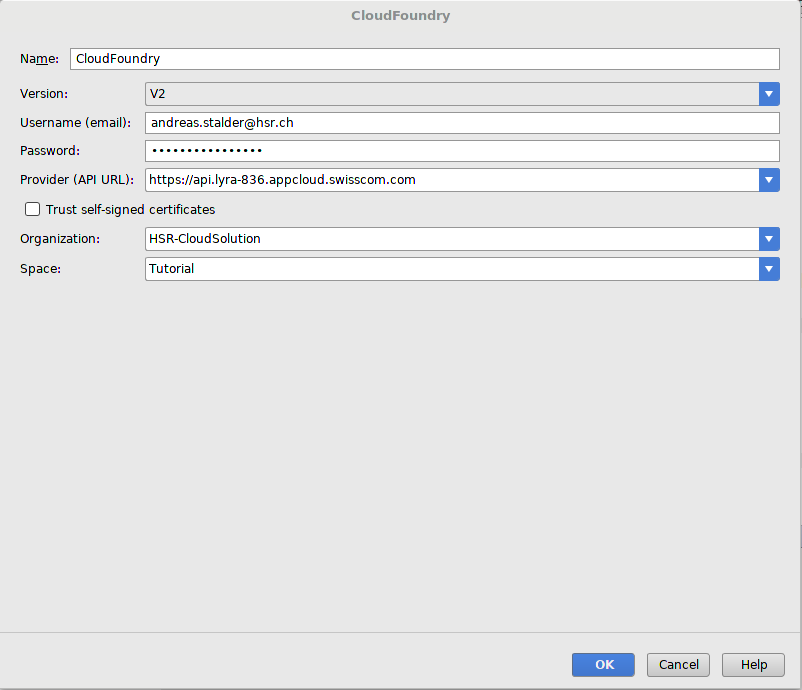
\includegraphics[width=0.65\columnwidth, valign=T]{images/cloudfoundryplugin.png}\\ \hline

Nun wird die Applikation gebuildet und auf die Swisscom-Cloud geladen. Wie man sieht, wird sofort eine Instanz erstellt und die Applikation ist erreichbar.
&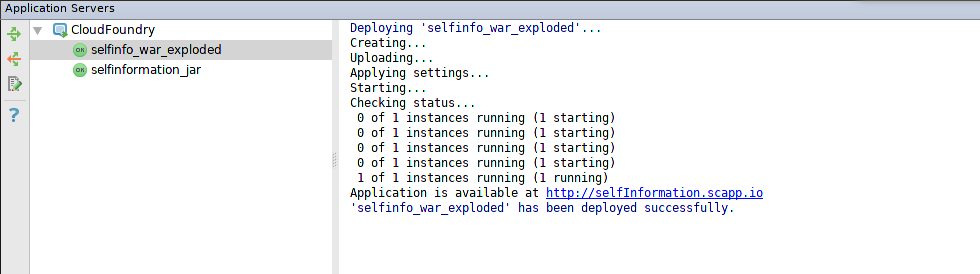
\includegraphics[width=0.65\columnwidth, valign=T]{images/instanzen.png}\\ \hline


Hier sieht man nun, dass die Applikation bereits erreichbar ist.
&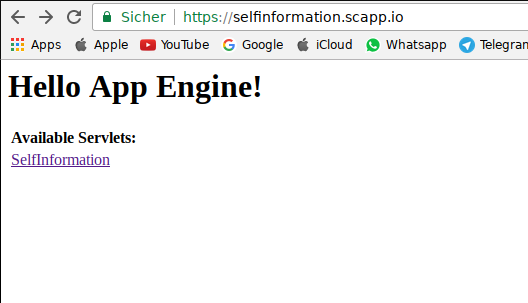
\includegraphics[width=0.65\columnwidth, valign=T]{images/laufendepp.png}\\ \hline
\end{longtable}
\section{Fragen}
\subsection{Wieviel RAM steht Ihrer Cloud-Instanz maximal zur Verfügung?}
Der Cloud-Instanz steht bei der Swisscom maximal 2 GB zur Verfügung. Mehr kann man leider nicht zuweisen.
Die App zeigt aber dies hier an:
\begin{itemize}
\item		Maximum memory (megabytes): 1276
\item		Total memory (megabytes): 1276
\item		Total space (megabytes): 1007
\item		Free space (megabytes): 854
\item		Usable space (megabytes): 787
\end{itemize}
Wie es aussieht, kann die Applikation nicht die ganzen 2 GB nutzen. Vielleicht wird dies aber auch dynamisch angepasst.
\subsection{Von welchem Hersteller stammt die JVM?}
\begin{itemize}
\item		java.runtime.name: OpenJDK Runtime Environment
\item		java.vm.version: 25.111-b14
\item		java.vm.vendor: Oracle Corporation
\item		java.vm.name: OpenJDK 64-Bit Server VM
\end{itemize}
Die VM stammt von Oracle. Es wird das OpenJDK auf einem Linuxserver verwendet.
\subsection{Welche IP-Adresse hat der Server laut der Self Information-Applikation?}
\begin{itemize}
\item		Name 0: w9a98pllh480-1
\item		InetAddresses 0: /10.254.0.138
\item		Name 1: lo
\item		InetAddresses 1: /127.0.0.1
\end{itemize}
Es sind zwei Interface verbunden. Das Loopback und eines mit dem Namen: w9a98pllh480-1. Die IP-Adresse ist 10.254.0.138. 
\chapter{Preisrecherche}
Swisscom verfolgt eine usage-based Pricing Strategie. Man bezahl also nur für laufende Dienst Die Kosten setzen sich zusammen aus den Ressourcen für die App + zusätzliche Services. Seit Ende 2016 wird bei der Swisscom stündlich abgerechnet. Davor wurde in täglichen Intervallen abgerechnet. Die Preise sind einfachheitshalber aber meist in CHF pro Monat angegeben. 

Für die Datenbankprodukte (MariaDB, MongoDB) hat Swisscom die Instanzen in drei verschiedenen Grössen kreiert (S, M, L). Man kann pro Grösse bis zu 10 Instanzen verwenden. 

Bei RabbitMQ bezahlt man Messages pro Monat. Für 1 Mio. Messages bezahlt man CHF 13.20.-. 

Für Diskspace bezahlt man einen Basispreis von CHF 9.00.-, damit hat man 100GB zur Verfügung. Für jede weiteren 100GB muss man zusätzliche CHF 6.00.- bezahlen.

Das Pricing für die Apps ist sehr einfach gehalten. Man hat nur 2 Faktoren, welche den Preis beeinflussen, nämlich Instanzen und Memory. Man bezahl pro 64MB CHF 1.50.- pro Monat. Die Instanzen dienen als Faktor. Wählen wir beispielsweise für unsere Applikation 512MB mit 2 Instanzen, so kostet uns das \((512MB/64MB)*1.50CHF*2=24CHF\) monatlich.

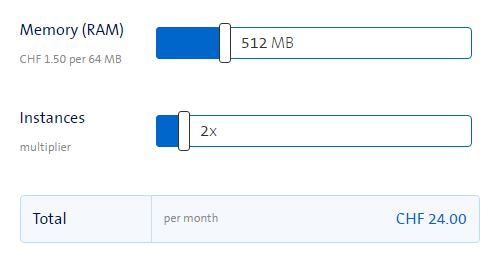
\includegraphics[scale=0.8]{images/pricepermonth.png}

Vor der Erstellung einer App muss dem Account eine Kreditkarte hinterlegt werden. Eine Bezahlung auf Rechnung ist in der Public Application Cloud nicht möglich.

Für neue User steht eine \glqq Welcome Offer\grqq zur Verfügung. Für die erste 3 Monate werden kosten bis CHF 100.00.- pro Monat erlassen. So kann man als Interessent ausgiebig testen. 

Die Preispolitik ist bei der Swisscom Application Cloud viel einfacher als bei AWS EC2. Die geforderte Konfiguration lässt sich weder mit Swisscom, noch mit AWS so einfach berechnen. Wir gehen nun von einer anderen Konfiguration aus:
\begin{itemize}
\item 2 Instanzen
\item 512MB RAM pro Instanz
\item 20GB Diskspace
\end{itemize}

Bei Swisscom kostet eine solche Konfiguration CHF 33.00.- monatlich. Bei AWS EC2 USD 11.44. Selbst wenn man die Währungsvorteile vom amerikanischen Dollar aussen vor lässt, ist Amazon doch sehr deutlich günstiger. Der Vergleich ist aber sehr gewagt, da bei Swisscom nicht ersichtlich ist, welche Computing Leistung man erhält. Bei AWS EC2 erhält man für diesen Preis eine sehr schwache CPU Leistung.

\chapter{Preisvergleich Hosting vs IaaS vs PaaS}
\chapter{Twelve-Factor Apps}
Als Beispielapplikation haben wir Das Miniprojekt aus WED2 vom Jahr 2016 genommen. Dies ist eine kleine Notizenapp in Node.JS geschrieben.
\section{Welche Anpassungen müssten Sie an Ihrer Applikation vornehmen?}
\subsubsection{Codebase}
Bei der Entwicklung der Notizenapp haben wir immer mit GitHub gearbeitet, da wir mehrere Entwickler waren. Da es eine kleine App war, haben wir aber immer nur ein Deploy geführt. Die Auftrennung in verschiedene Deploys war zu diesem Zeitpunkt noch nicht nötig, aber wäre schnell umsetzbar. Daher muss bei diesem Punkt nichts angepasst werden. 
\subsubsection{Dependencies}
Da die App in Node geschrieben wurde, konnten wir bei den Dependencies auf npm zurückgreifen. In unserer package.json Datei gab es ein dependencies Bereich mit allen Abhängigkeiten.
\subsubsection{Config}
Eine eigene Konfigurationsdatei gab es bei uns nicht. Dies müsste man für den 12-Faktoren Check eingebaut werden. Die Datenbankanbindung könnte sicher in diese Konfigurationsdatei, sowie auch die Servereinstellungen, wie der Port usw.
\subsubsection{Backing services}
Bei der Beispielapplikation wurde ein Backing services verwendet. Die Datenbank wurde zu Redis ausgelagert, damit man keinen lokalen Speicher verwenden musste. 
\subsubsection{Build, release, run}
Wir haben keine Aufteilung in Build und Releases gemacht, da dies bei Node nicht üblich ist. Um dies einzurichten, könnte man Heroku Buildpack für Node.js einrichten, damit man verschiedene Build hat. Weiter kann man via npm Parameter angeben, welcher Stand der Release hat. Zum Beispiel so: ''npm install --production''. Dies wurde aber nicht gemacht.
\subsubsection{Processes}
Da wir nur ein Miniprojekt entwickelt haben, haben wir diesen Punkt nicht eingerichtet. Aber Dies ist bei Node kein Problem. Unter Linux kann man einfach eine Systemd Service Konfigurationsdatei erstellen. Dieser wird in den Autostart verlinkt und so startet die Applikation immer in einem eigenen Service. Da die Daten in einer Datenbank gespeichert wurden, war die Applikation auch Stateless und konnte mehrmals gestartet werden.
\subsubsection{Port binding}
Port Binding ist bei Node immer der Fall, da es sich bei Node um einen Webserver handelt. Bei unserem Beispiel konnten wir den Port 3000 einstellen. Das Port Binding könnte auch noch per Konfigurationsdatei für die Verschiedenen Bereiche (Development oder Running System) separat angegeben werden.
\subsubsection{Concurrency}
Durch das asynchrone System von Node und ohne grössere Backgroud Tasks, ist Concurrency ziemlich einfach. Einzig der Datenbankzugriff müsste wohl noch Concurrent gmacht werden, damit es bei der Datenbank nicht zu Race Conditions kommt.
\subsubsection{Disposability}
Unsere Applikation unterstützt diesen Punkt. Node startet extrem schnell und die HTTP Requests sind auch kurz. Daher ist dieser Punkt bei so kleinen Node Projekten einfach erreichbar.
\subsubsection{Dev/Prod parity}
Da wir hier keine Trennung hatten, da es sich nur um ein Miniprojekt handelte, ist uns dies gelungen. Bei einer Weiterentwicklung würde man dafür auf verschiedenen Branches auf GitHub arbeiten.
\subsubsection{Logs}
In unserem Projekt wurde im Endprodukt kein Log eingebaut. Dies müsste noch eingebaut werden, damit man den 12-Faktor Standard erreicht. Im npm-Repo gibt es gute Logging Lösungen, welche dies einfach implementierbar machen.
\subsubsection{Admin processes}
Admin Tasks werden bei Node, wie auch bei unserem Projekt in das /bin Verzeichnis verschoben. Danach wird mit eigenen Scripts gearbeitet, welche die Tasks im Laufenden Betrieb erledigen. Durch das schnelle starten von Node, sollte das kein Problem sein.
\section{Wie untterscheidet sich diese Methode von IDEALen nach Fehling et al?}
Im Grunde wollen beide Methoden das selbe. 12-Faktor zeigt dies einfach in mehreren kleinen Kapiteln, anstelle von fünf grossen Kapiteln. 
Was aber im IDEAL fehlt oder weniger genau beschrieben ist, sind folgende Kapitel aus der 12-Faktor Methode:
\begin{itemize}
\item	Codebase
\item	Build, release, run
\item	Port Binding
\item	Disposability
\item	Dev/prod partity
\item	Logs
\item	Admin processes
\end{itemize}
\section{Welche der beiden Methoden scheint einfacher?}
Die 12-Faktor Methode scheint mir einfacher zu sein. Diese ist viel genauer beschrieben und man weiss bei jedem Punkt genau, was man anpassen muss.









